\section{1926 The wheel of Life Issue}

\lettrine{T}{uva's stamps}, even today present a puzzle. Firstly the monetary system of the country was the lan and aksha, the latter apparently from an old Turkish coin. The first series depicted the Buddhist wheel of life with Mongolian writing and numerals only, representing the value in lan and aksha.
\footnote{According Postal Services of Tuva.} 

\begin{fullwidth}
\begin{figure}[htp]
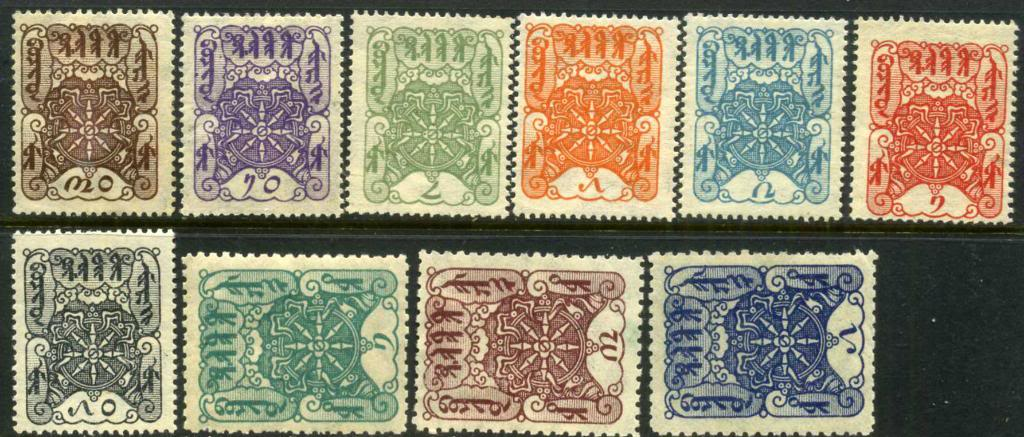
\includegraphics[width=.95\textwidth]{../tannu-tuva/1926-set.jpg}
\caption{Tannu Tuva 1926. Sc. 1-10. MLHOG. SCV \$40.25  \$50}
\end{figure}
\end{fullwidth}

Between 1926 and 1933, Tannu Tuva issued 38 postage stamps.\footnote{According to Scott Catalogue.}






                                                                      